\documentclass[tikz,border=2mm]{standalone}
\usetikzlibrary{positioning}
\usepackage{amssymb}
\definecolor{structure}{HTML}{1A535C}   % Deep Teal
\definecolor{main}{HTML}{C6892A}        % Golden Ochre
\definecolor{second}{HTML}{2E4057}      % Slate Blue
\definecolor{third}{HTML}{8B2635}       % Burgundy

\begin{document}

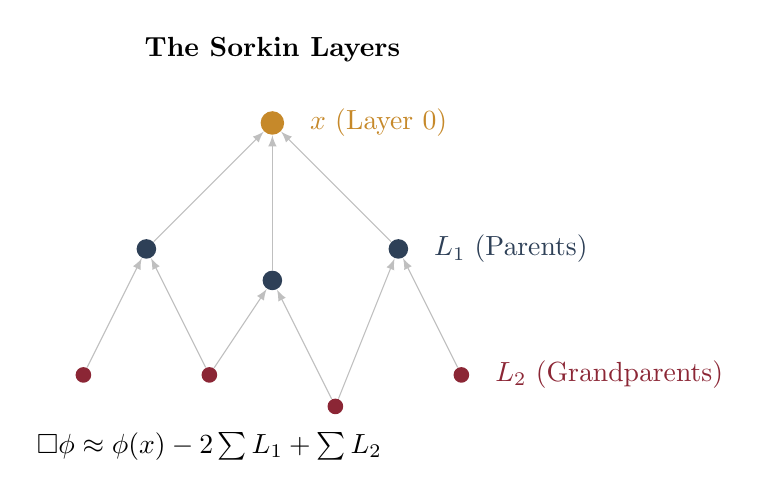
\begin{tikzpicture}[
    scale=0.8,
    node distance=1.5cm,
    event/.style={circle, fill=structure, inner sep=2pt},
    layer0/.style={circle, fill=main, inner sep=3pt},
    layer1/.style={circle, fill=second, inner sep=2.5pt},
    layer2/.style={circle, fill=third, inner sep=2pt},
    link/.style={draw=gray!50, thin, ->, >=latex}
]

% The Event x
\node[layer0] (x) at (0, 0) {};
\node[right=2mm of x, color=main] {$x$ (Layer 0)};

% Layer 1 (Parents)
\node[layer1] (y1) at (-2, -2) {};
\node[layer1] (y2) at (0, -2.5) {};
\node[layer1] (y3) at (2, -2) {};
\node[right=2mm of y3, color=second] {$L_1$ (Parents)};

% Links L1 -> L0
\draw[link] (y1) -- (x);
\draw[link] (y2) -- (x);
\draw[link] (y3) -- (x);

% Layer 2 (Grandparents)
\node[layer2] (z1) at (-3, -4) {};
\node[layer2] (z2) at (-1, -4) {};
\node[layer2] (z3) at (1, -4.5) {};
\node[layer2] (z4) at (3, -4) {};
\node[right=2mm of z4, color=third] {$L_2$ (Grandparents)};

% Links L2 -> L1
\draw[link] (z1) -- (y1);
\draw[link] (z2) -- (y1); \draw[link] (z2) -- (y2);
\draw[link] (z3) -- (y2); \draw[link] (z3) -- (y3);
\draw[link] (z4) -- (y3);

% Extra Links L2 -> L0 (Transitivity) - but Layers definition usually excludes direct parents?
% Sorkin layers are defined recursively. 
% L1 = Maximal elements of Past(x)
% L2 = Maximal elements of Past(x) \ L1
% So direct links z -> x are possible but z is not maximal in Past(x) because y is between.
% Transitivity is implied. We visualize the Hasse diagram (transitive reduction).

% Environment label
\node[above=0.5cm of x] {\textbf{The Sorkin Layers}};
\node[below=0.5cm of z2] {$\square \phi \approx \phi(x) - 2 \sum L_1 + \sum L_2$};

\end{tikzpicture}

\end{document}
